\section{Clustering using \acs{optics}}\label{sec:evaluation-OPTICS}
% OPTIC cluster results
\begin{figure}[!htb]%
    \centering
    \subfloat[\centering Preprocessing according to \autoref{pt:32} (cf. \cite{OPTICS1999}).]{{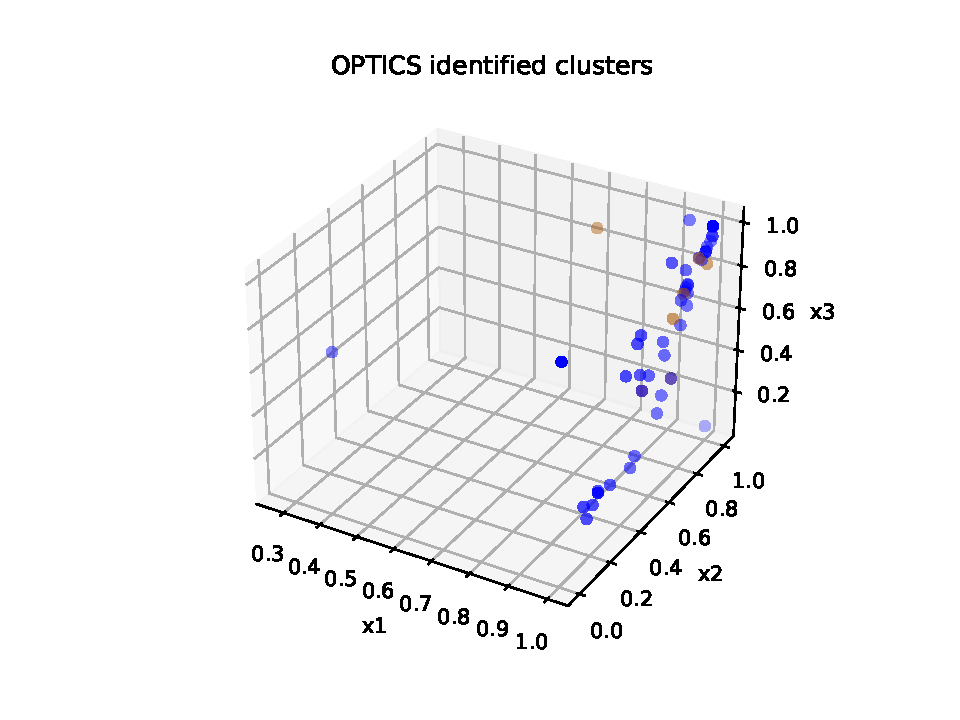
\includegraphics[width=6.5cm]{images/OPTICS/32x32/OPTICS_cluster_32x32.pdf} }}%
    \qquad
    \subfloat[\centering Preprocessing according to \autoref{pt:eigendocs} (i.e.\ \eigendocs{}).]{{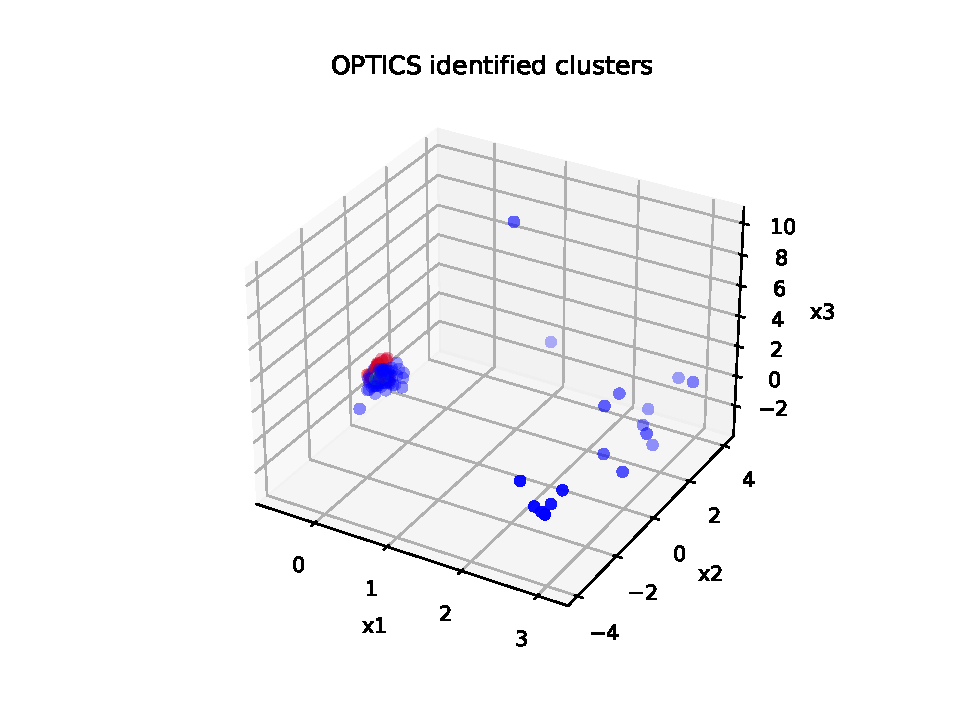
\includegraphics[width=6.5cm]{images/OPTICS/eigendocs/OPTICS_cluster_eigendocs.pdf} }}%
    \caption[\ac{optics} clusters]{The clusters are extracted from the respective reachability plots in \autoref{fig:reachability_plots} by \ac{optics}.
    The blue points are noise points, whereas any other colour denotes a cluster.}%
    \label{fig:optics_cluster}%
\end{figure}

% 3d plots
The algorithm \ac{optics} is applied to data, which is preprocessed according to \autoref{pt:32} and \autoref{pt:eigendocs}.
The clusters from \autoref{fig:optics_cluster} are extracted from the respective reachability plots in \autoref{fig:reachability_plots}.
The three-dimensional plots visualize the first three dimensions of the data and thus, the weights of the first three principal components assigned by the \eigendocs{} algorithm.
By visual inspection and comparison of both plots, 
it can be seen that the projection by the \eigendocs{} approach of \autoref{pt:eigendocs} scatters the objects further in the three-dimensional space.
One could argue that this is due to the fact, 
that the input data encodes not only the visual appearance in terms of page layout but also the size of the document.
Possibly, the objects are grouped by document size.


% cluster content
To analyze the results of the clustering, the content of the clusters is examined.
Since the documents are not labeled, the content of the clusters is analyzed by visual inspection.
The content of the clusters is displayed in \autoref{fig:optics_content_cluster}.
The yellow images belong to the group identified as noise.
The images preprocessed according to \autoref{pt:32} are partitioned into more clusters than the \eigendocs{} approach.
Most of the certificates are classified as noise for both approaches.

\begin{figure}[!htb]%
    \centering
    \subfloat[\centering Preprocessing according to \autoref{pt:32} (cf. \cite{OPTICS1999}).]{{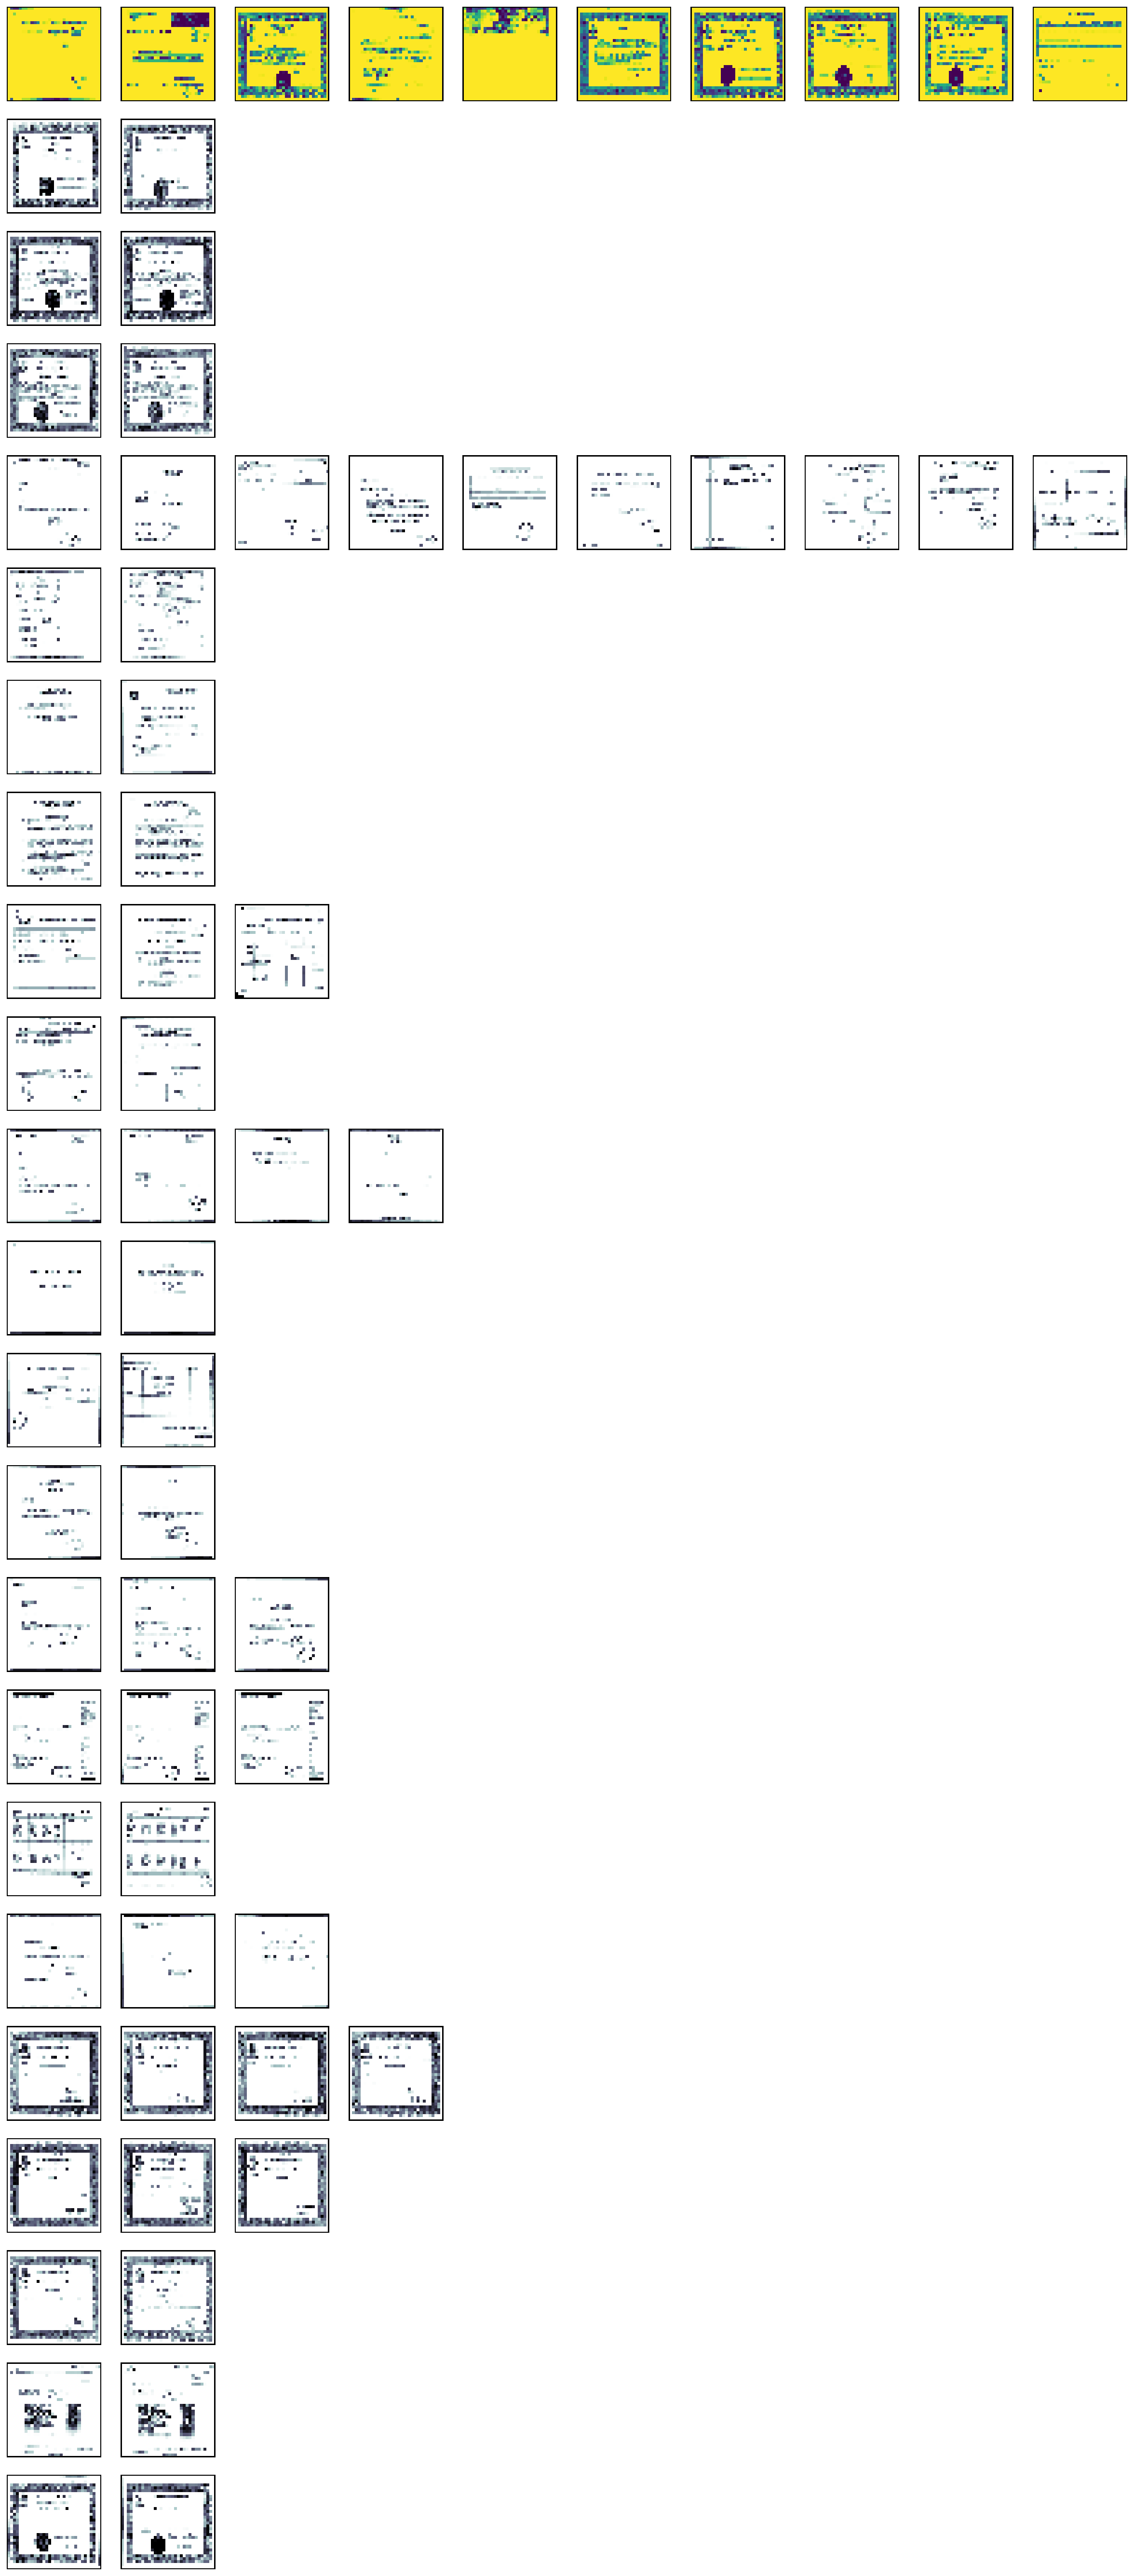
\includegraphics[width=6.5cm]{images/OPTICS/32x32/cluster_content_noise_32x32.pdf} }}%
    \qquad
    \subfloat[\centering Preprocessing according to \autoref{pt:eigendocs} (i.e.\ \eigendocs{}).]{{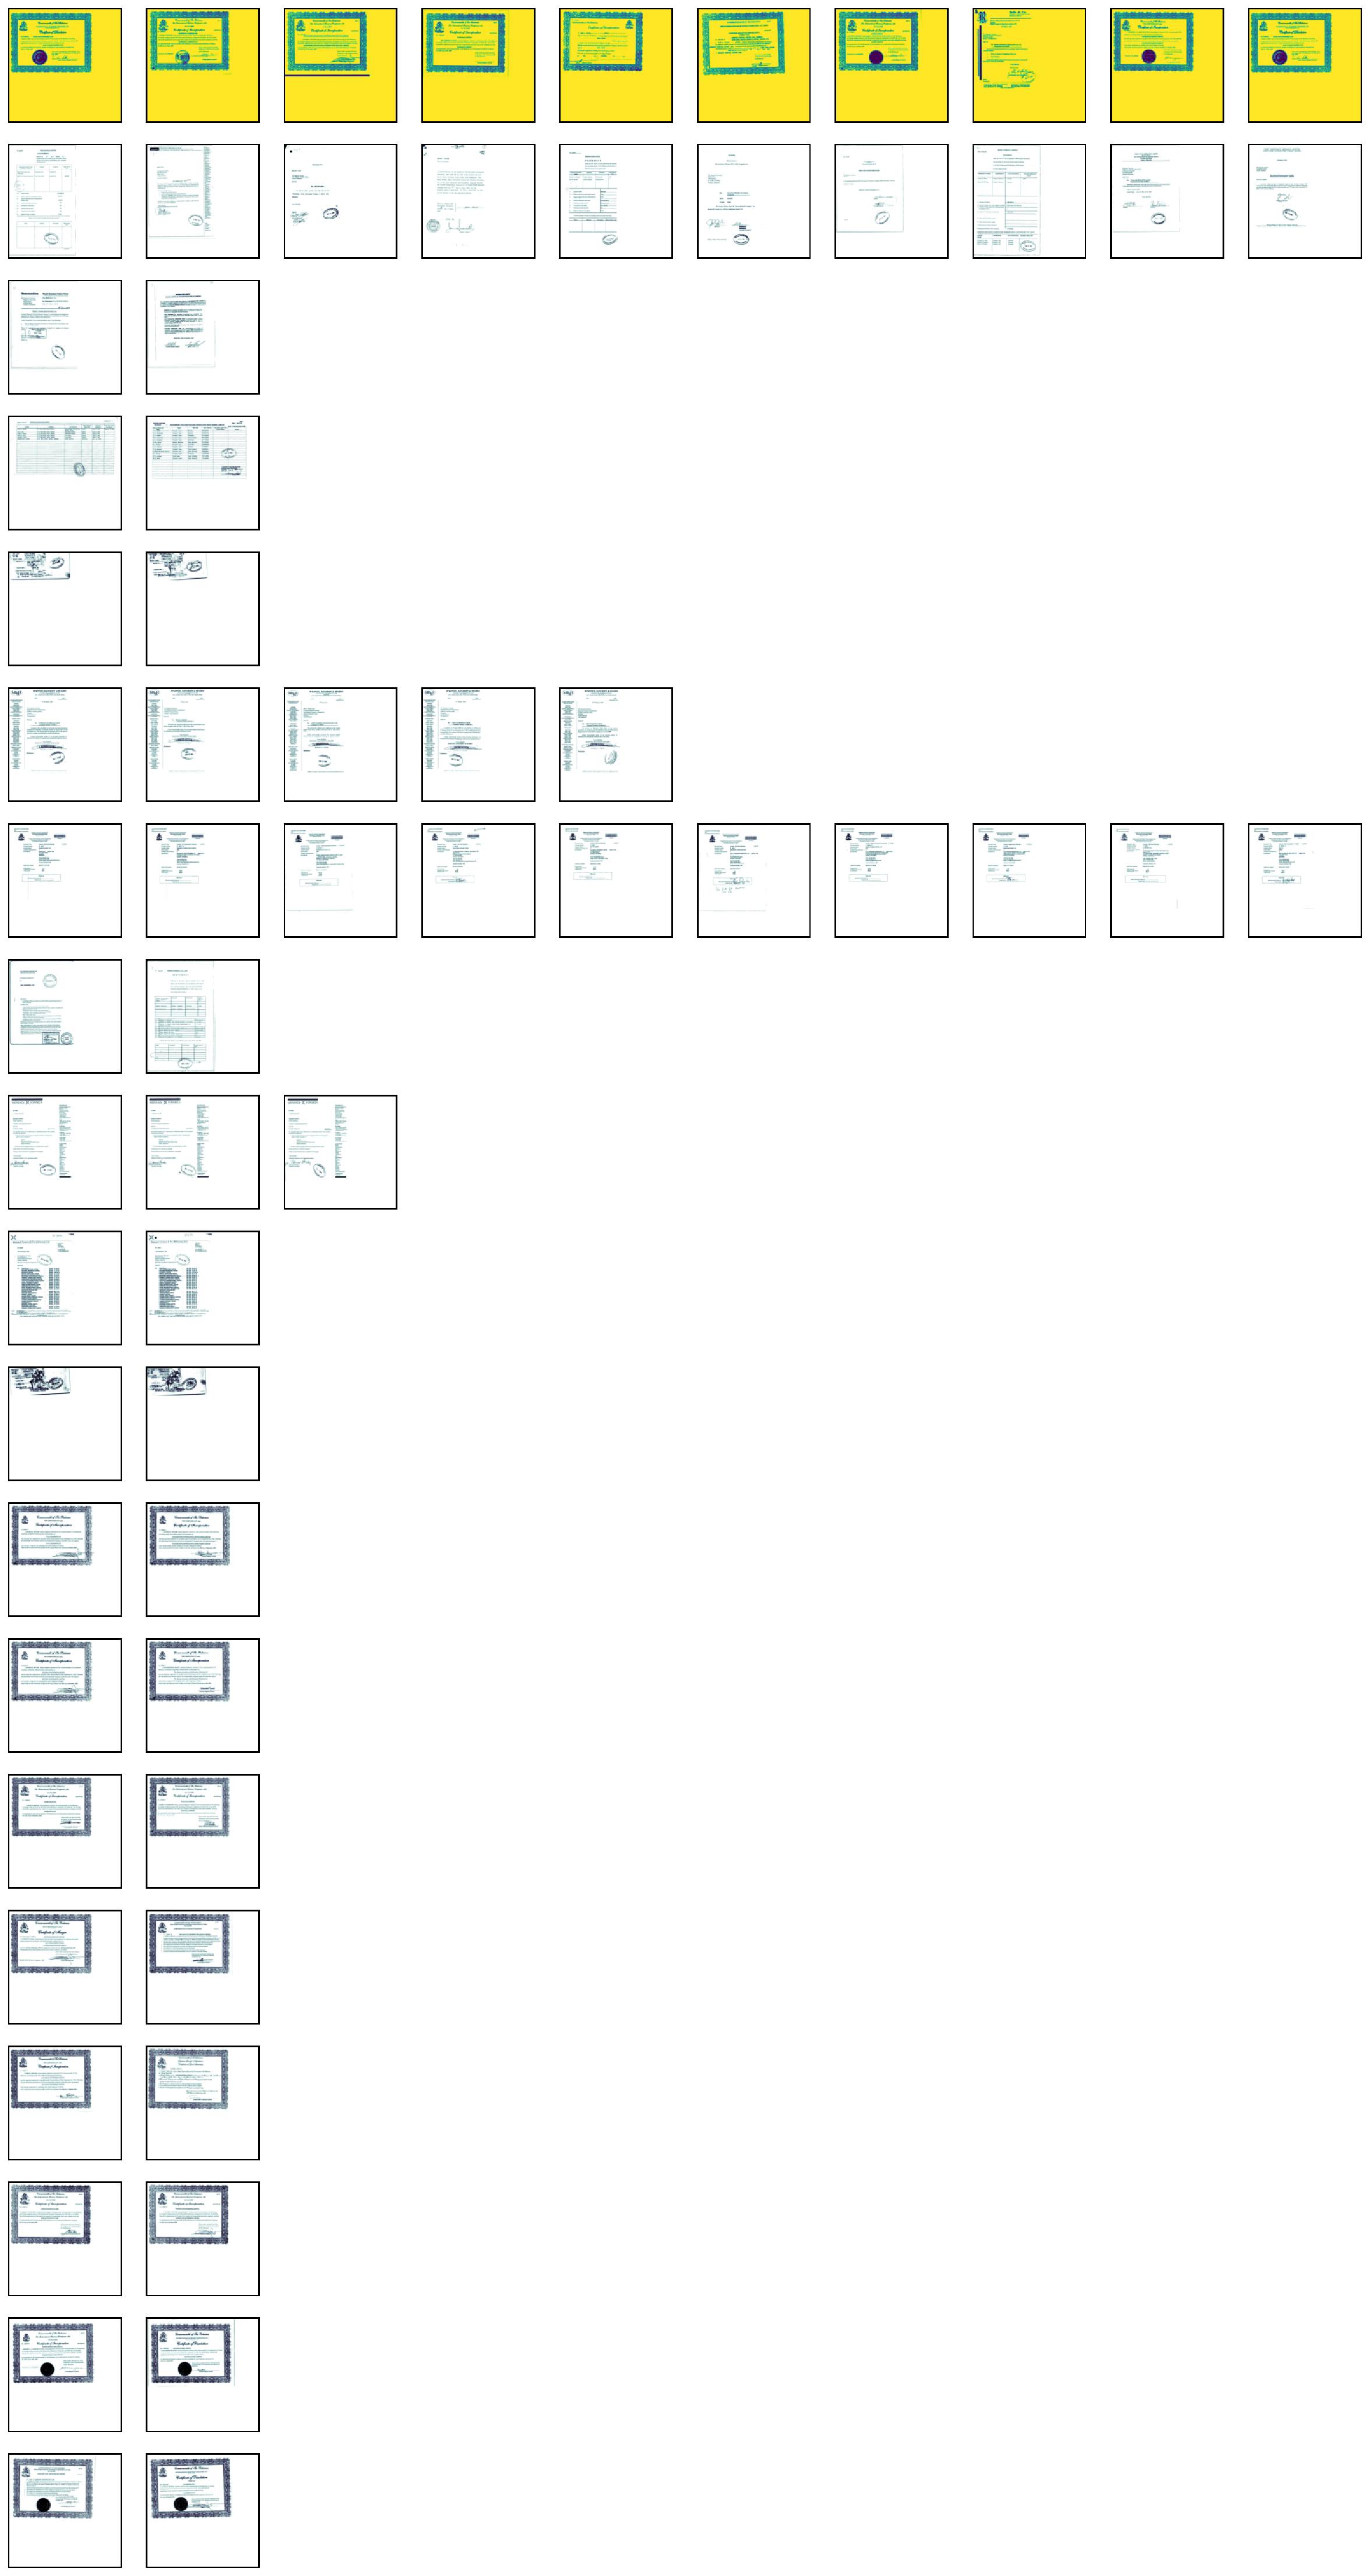
\includegraphics[width=6.5cm]{images/OPTICS/eigendocs/cluster_content_noise_eigendocs.pdf} }}%
    \caption[\ac{optics} clusters]{In this visualization, at most 10 random elements of a cluster are displayed.
    The yellow images belong to the group denoted as noise.
    Most certificates are classified as noise.
    }%
    \label{fig:optics_content_cluster}%
\end{figure}


The preprocessing approach used to create the \ac{optics} input for the \databaseName{} database index is \eigendocs{} 
since it also encodes information about the document size. 

% code
According to \citeauthor{OPTICS2014}, \ac{optics} was developed to improve \ac{dbscan} flaws.
With respect to the evolution of these clustering methods, i.e.\ \ac{dbscan} being \ac{optics} basis, 
\ac{dbscan} is chosen for the cluster method in \lst{lst:optics_model}.
In order to reduce calculation complexity the maximum $\varepsilon$ is 10.
The distance between two points to still be considered neighbours is defined after a visual inspection of the reachability plot.
Considering the intrinsic structure of the \eigendocs{} data it is set to $1.5$ to return meaningful clusters.